\label{chapter:projeto}

\par
\textcolor{red}{Os dado...}

\section{Pré-processamento}

\par
\textcolor{red}{Com os dados mencionados anteriormente, foram fornecidos no formato de arquivo .xlsx do Excel com uma tabela contendo três colunas de informações com o ID do candidato, a resposta do questionario e o número do questionario atribuido a resposta, como demonstrado na Figura 19. De 37 questões, somente 33 poderam ser fornecidas, pois, quatro delas tinham como respostas dissertativas e apenas as 33 tinham como resposta opções já fornecidas pelo próprio sitema que davam de armazenar no banco de dados.}

\par
\begin{figure}[!htp]
	\begin{center}
    \caption{\label{fig:waveform_fig} Dados fornecidos pela CPV.}
	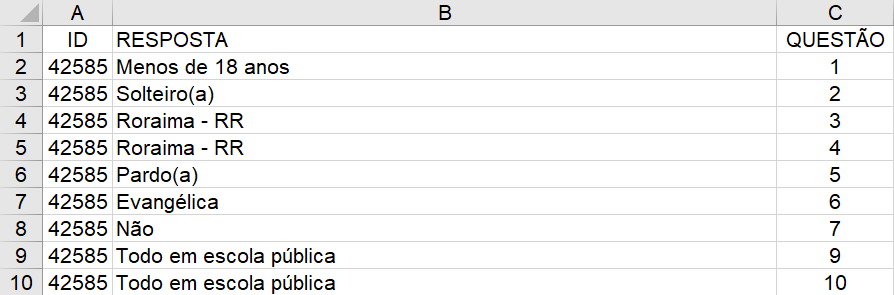
\includegraphics[scale=0.65]{Figuras/Formato_errado.png}
	\end{center}
    \legend{Fonte: Próprio autor.}
\end{figure}

\par
\textcolor{red}{Para poder começar com a utilização desses dados, foi necessário transformar toda a tabela para um formato apropriado a fim de que os aplicativos do software WEKA os suporte. De inicio foi feito colunas para cada número do questionário através das funções de filtro e concatenção fornecida pelo Excel, e as linhas abaixo delas seriam as respostas de cada candidato para aquela coluna especifica, como demonstrado na Figura 20. A coluna de ID foi removida já que não era necessario para a mineração, entretanto, ela foi necessaria na geração de uma coluna nova rotulada de Aprovado que foi abtida através de duas tabelas contendo informações dos candidatos geral e dos de aprovados.}

\par
\begin{figure}[!htp]
	\begin{center}
    \caption{\label{fig:waveform_fig} Tabela depois de formatada.}
	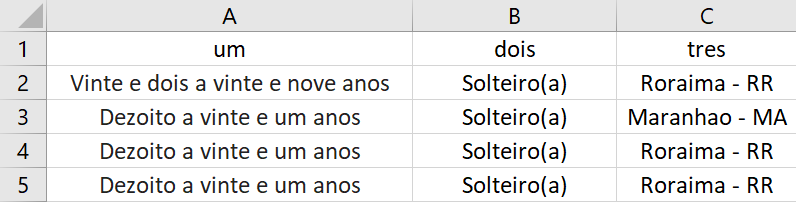
\includegraphics[scale=0.65]{Figuras/Formato_certo.png}
	\end{center}
    \legend{Fonte: Próprio autor.}
\end{figure}

\par
\textcolor{red}{O motivo dessa formatação é que o WEKA identifica a primeira linha como atributos e as linhas subsequentes os dados relacionados a eles.}

